\part{The Middleware Architecture:\\UObjects}
\label{sec:tut:uobject}

\chapter*{Introduction}
This part guides you through the various steps of writing an \urbi
\Cxx component using the UObject API. This API can be used to add new
objects written in \Cxx to the \urbi language, and to interact from
\Cxx with the objects that are already defined. We cover the use cases
of controlling a physical device (servomotor, speaker, camera...), and
interfacing higher-lever components (voice recognition, object
detection, ...) with \urbi.

The API defines the UObject class. Each instance of a derived class in
your \Cxx code will correspond to an \urbi object sharing some of its
methods and attributes. The API provides methods to declare which
elements of your object are to be shared. To share a variable with
\urbi, you have to give it the type UVar. This type is a container that
provides cast and equal operators for all types known to \urbi: double,
string and char*, and the binary-holding structures UBinary, USound
and UImage. This type can also read from and write to the liburbi
UValue class. The API provides methods to set up callbacks functions
that will be notified when a variable is modified or read from \urbi
code. Instance methods of any prototype can be rendered accessible
from \urbi, providing all the parameters types and the return type can
be converted to/from UValue.

The next section is a walk through covering all the aspects of the
UObject API, and the rest of the chapter describes many use cases in
details.

\newenvironment{todo}{%
  \begin{quote}\itshape%
  }{%
  \end{quote}%
}

\chapter{Quick Start}
\label{sec:uob:quick}

This chapter presents \urbi SDK with a specific focus on its
middleware features.  It is self-contained in order to help readers
quickly grasp the potential of \urbi used as a middleware.  References
to other sections of this document are liberally provided to point the
reader to the more complete documentation; they should be ignored
during the first reading.

\section{\urbi as Middleware}

\urbi SDK is meant to make easier the orchestration of independent,
concurent, components.  It was first designed for robotics: it
provides all the needed features to coordonate the execution of
various components (actuators, sensors, software devices that provide
features such as text-to-speach, face recognition and so forth).
Traditional languages such as \Cxx are definitely very adequate to
program the local, low-level, handling of these hardward or software
devices; indeed one needs efficiency, small memory footprint, and
access to low-level hardware details.  Yet, when it comes to
orchestration and to coordination between components, in a word, when
it comes to \emph{address concurrency}, such languages are no longer
an adequate model.

Rather, one has to select a middleware infrastructure in order to be
able to use remote components as if they were local, to allow
concurrent execution, to make synchronous or asynchronous requests and
so forth.  The \dfn{UObject} architecture provide exactly this: a
common API which allows conformant components to be used seemlessly in
highly concurrent settings.  Components need not be designed with
UObjects in mind, rather, UObjects are typically ``shells'' around
``regular'' components.

As a quite magical feature that comes for free, components with an
UObject interface are naturally supported by the \us programming
language.  This can be a tremendous help: one can interact with these
components (making queries, changing them, observing their state,
monitoring various kinds of events and so forth), which provides a
huge speed-up during development.

Finally, note that, although made with robots in mind, the UObject
architecture is well suited to tame any heavily concurrent
environment, such as video games.

\subsection{The \urbi Architecture}

\begin{todo}
  * Description approche Urbi, philosophie (orchestration etc) => un
  exemple de code Urbiscript qui orchestre 3 UObject de manière simple
  mais non triviale, avec at, \&, events, tags et qui servira de fil
  conducteur au quickstart (le but du quickstart est de refaire cet
  exemple initial).
\end{todo}

\section{UObject Basics}

As a simple running example, consider a (very) basic factory.  Raw
material delivered to the factory is push into some assembly machine,
which takes some time.

As a firth component of this factory, consider the following
implementation of the core engine of the factory.
\newcommand{\factoryDir}{\uobjectsDir/factory/factory.uob}
\lstinputlisting[language=C++,basicstyle=\ttfamily\footnotesize]{\factoryDir/factory.hh}
\lstinputlisting[language=C++,basicstyle=\ttfamily\footnotesize]{\factoryDir/factory.cc}

\subsection{Wrapping into an UObject}

By \dfn{binding} a UObject, we mean using the UObject API to declare
objects to the Urbi world.  These objects have member variables (also
known as \dfn{attributes}) and/or member functions (also known as
\dfn{methods}) all of them or some of them being declared into the
Urbi world.

One could modify the \lstinline|Factory| class to make it a UObject,
yet we rather recommend wrapping pure \Cxx classes into a UObject.  It
is strongly suggested to aggregate the native \Cxx objects in the
UObject --- rather than trying to derive from it.

\lstinputlisting[language=C++,basicstyle=\ttfamily\footnotesize]{\factoryDir/ufactory.hh}

The implementation of \lstinline|UFactory| is quite straightforward.
It uses some of the primitives used in the binding process
(\autoref{sec:uob:api:bind}):
\begin{itemize}
\item \lstinline|UStart(\var{class})| declares classes that are
  UObjects; eventually, such classes will appear in \us as
  \lstinline|uobjects.\var{class}|.  Use it once.

\item \lstinline|UBindFunction(\var{class}, \var{function})| declares
  a \var{function}.  Eventually bound in the \us world as
  \lstinline|uobjects.\var{class}.\var{function}|.

\item Similarly, \lstinline|UBindVar(\var{class}, \var{variable})|
  declares a \var{variable}.
\end{itemize}

\urbi relies on the prototype model for object-oriented programming,
which is somewhat different from the traditional \Cxx class-based
model (\autoref{sec:tut:value}).  This is reflected by the presence of 
\emph{two} different constructors:
\begin{itemize}
\item \lstinline|UFactory::UFactory|, the \Cxx constructor which is
  invoked for every single instance of the UObject.  It is always
  invoked by the \urbi system when instantiating a UObject,
  \emph{including} the prototype itself.  It sole argument is its name
  (an internal detail you need not be aware of), and its main purpose
  is to register attributes and functions, especially the
  \lstinline|UFactory::init| function.

\item \lstinline|UFactory::init|, the \urbi constructor invoked each
  time a new clone of \lstinline|UFactory| is made, i.e., for every
  instance except the first one.
  
  Functions and variables that do not make sense for the initial
  prototype (which might not be fully functional) should be bound
  here, rather that in the \Cxx constructor.
\end{itemize}

The following listing is abundantly commented, and is easy to grasp.

\lstinputlisting[language=C++,basicstyle=\ttfamily\footnotesize]{\factoryDir/ufactory.cc}

\subsection{Asynchronicity}
\begin{todo}
  * Asynchronisme dans UObject: notifychange, timers
\end{todo}

\subsection{Running Components}
\begin{todo}
  * Compilation et branchement de UObject (urbi-launch): expliquer les
  deux modes: distant / pluge'

  * Cycle complet de lancement d'une appli Urbi: lancement d'urbi,
  execution d'urbi.ini, chargement dynamique des UObjects
\end{todo}

\section{Using \us}

\subsection{The \us Scripting Language}
\begin{todo}
  * Introduction a` Urbiscript (rappeler que c'est avant tout un
  langage comme les autres, avec if/for/while, etc), puis passer
  rapidement aux elements clefs de la prog evenementielle dans Urbi:
  at/whenever
\end{todo}

\subsection{Concurrency}
\begin{todo}
  * Parallelisme explicite: \&

  * Tags et controle d'execution

  * Channels et liburbi (les principes, renvoyer a` la doc liburbi pour
  l'API)

  * All together, on reprend l'exemple du de'but et on de'taille le code
  des UObjects utilise's, puis le code urbiscript.
\end{todo}

\section{Conclusion}
\begin{todo}
  * Conclusion note: expliquer qu'on peut embedder l'engine Urbi dans
  une appli native C++ (tout le monde le demande), qu'on peut faire
  des bridges ge'ne'riques avec d'autres archis a` composants (citer
  CORBA), donner le lien pour te'le'charger, le lien vers la doc du
  langage urbiscript, vers la doc de UObject, etc.
\end{todo}


%%% Local Variables:
%%% mode: latex
%%% TeX-master: "../urbi-sdk"
%%% End:

%% Copyright (C) 2009-2010, Gostai S.A.S.
%%
%% This software is provided "as is" without warranty of any kind,
%% either expressed or implied, including but not limited to the
%% implied warranties of fitness for a particular purpose.
%%
%% See the LICENSE file for more information.

\chapter{The UObject API}
\label{sec:uob:api}

The UObject API can be used to add new objects written in \Cxx to the
\us language, and to interact from \Cxx with the objects that are
already defined. We cover the use cases of controlling a physical
device (servomotor, speaker, camera\ldots), and interfacing
higher-lever components (voice recognition, object detection\ldots)
with \urbi.

The \Cxx API defines the UObject class. To each instance of a \Cxx class
deriving from UObject
will correspond an \us object sharing some of its
methods and attributes. The API provides methods to declare which
elements of your object are to be shared. To share a variable with
\urbi, you have to give it the type UVar. This type is a container
that provides conversion and assignment operators for all types known to
\urbi: \lstinline{double}, \lstinline{std::string} and \lstinline{char*},
and the binary-holding structures
\lstinline{UBinary}, \lstinline{USound} and \lstinline{UImage}. This type
can also read from and write to
the liburbi UValue class. The API provides methods to set up callbacks
functions that will be notified when a variable is modified or read
from \urbi code. Instance methods of any prototype can be rendered
accessible from \us, providing all the parameters types and the return
type can be converted to/from UValue.

\section{Compiling UObjects}

UObjects can be compiled easily directly with any regular compiler.
Nevertheless, \usdk provides two tools to compile UObject seamlessly.

In the following sections, we will try to compile a shared library named
\file{factory.so} (or \file{factory.dll} on Windows platforms) from a set of
four files (\file{factory.hh}, \file{factory.cc}, \file{ufactory.hh},
\file{ufactory.cc}).  These files are stored in a \file{factory.uob}
directory; its name bares no importance, yet the \file{*.uob} extension
makes clear that it is a UObject.

In what follows, \var{urbi-root} denotes the top-level directory of your
\usdk package, see \autoref{sec:install:install}.

\subsection{Compiling by hand}

On Unix platforms, compiling by hand into a shared library is
straightforward:

\begin{shell}
$ g++ -I \var{urbi-root}/include \
      -fPIC -shared \
      factory.uob/*cc -o factory.so
$ file factory.so
factory.so: ELF 32-bit LSB shared object, Intel 80386, \
  version 1 (SYSV), dynamically linked, not stripped
\end{shell}

On Mac OS X the flags \option{-Wl,-undefined,dynamic\_lookup} are needed:

\begin{shell}
$ g++ -I \var{urbi-root}/include \
      -shared -Wl,-undefined,dynamic_lookup \
      factory.uob/*.cc -o factory.so
$ file factory.so
factory.so: Mach-O 64-bit dynamically linked shared library x86_64
\end{shell}

\subsection{The \command{umake-*} family of tools}

\command{umake} can be used to compile UObjects.  See
\autoref{sec:tools:umake} for its documentation.

You can give it a list of files to compile:
\begin{shell}
$ umake -q --shared-library factory.uob/*.cc -o factory.so
umake: running to build library.
\end{shell}

\noindent
or directories in which \Cxx sources are looked for:

\begin{shell}
$ umake -q --shared-library factory.uob -o factory.so
umake: running to build library.
\end{shell}

\noindent
or finally, if you give no argument at all, the sources in the current
directory:

\begin{shell}
$ cd factory.uob
$ umake -q --shared-library -o factory.so
umake: running to build library.
\end{shell}


\subsection{Using the Visual \Cxx Wizard}

If you installed \usdk using its installer, and if you had Visual \Cxx
installed, then the UObject wizard was installed.  Use it to create your
UObject code:

\begin{center}
  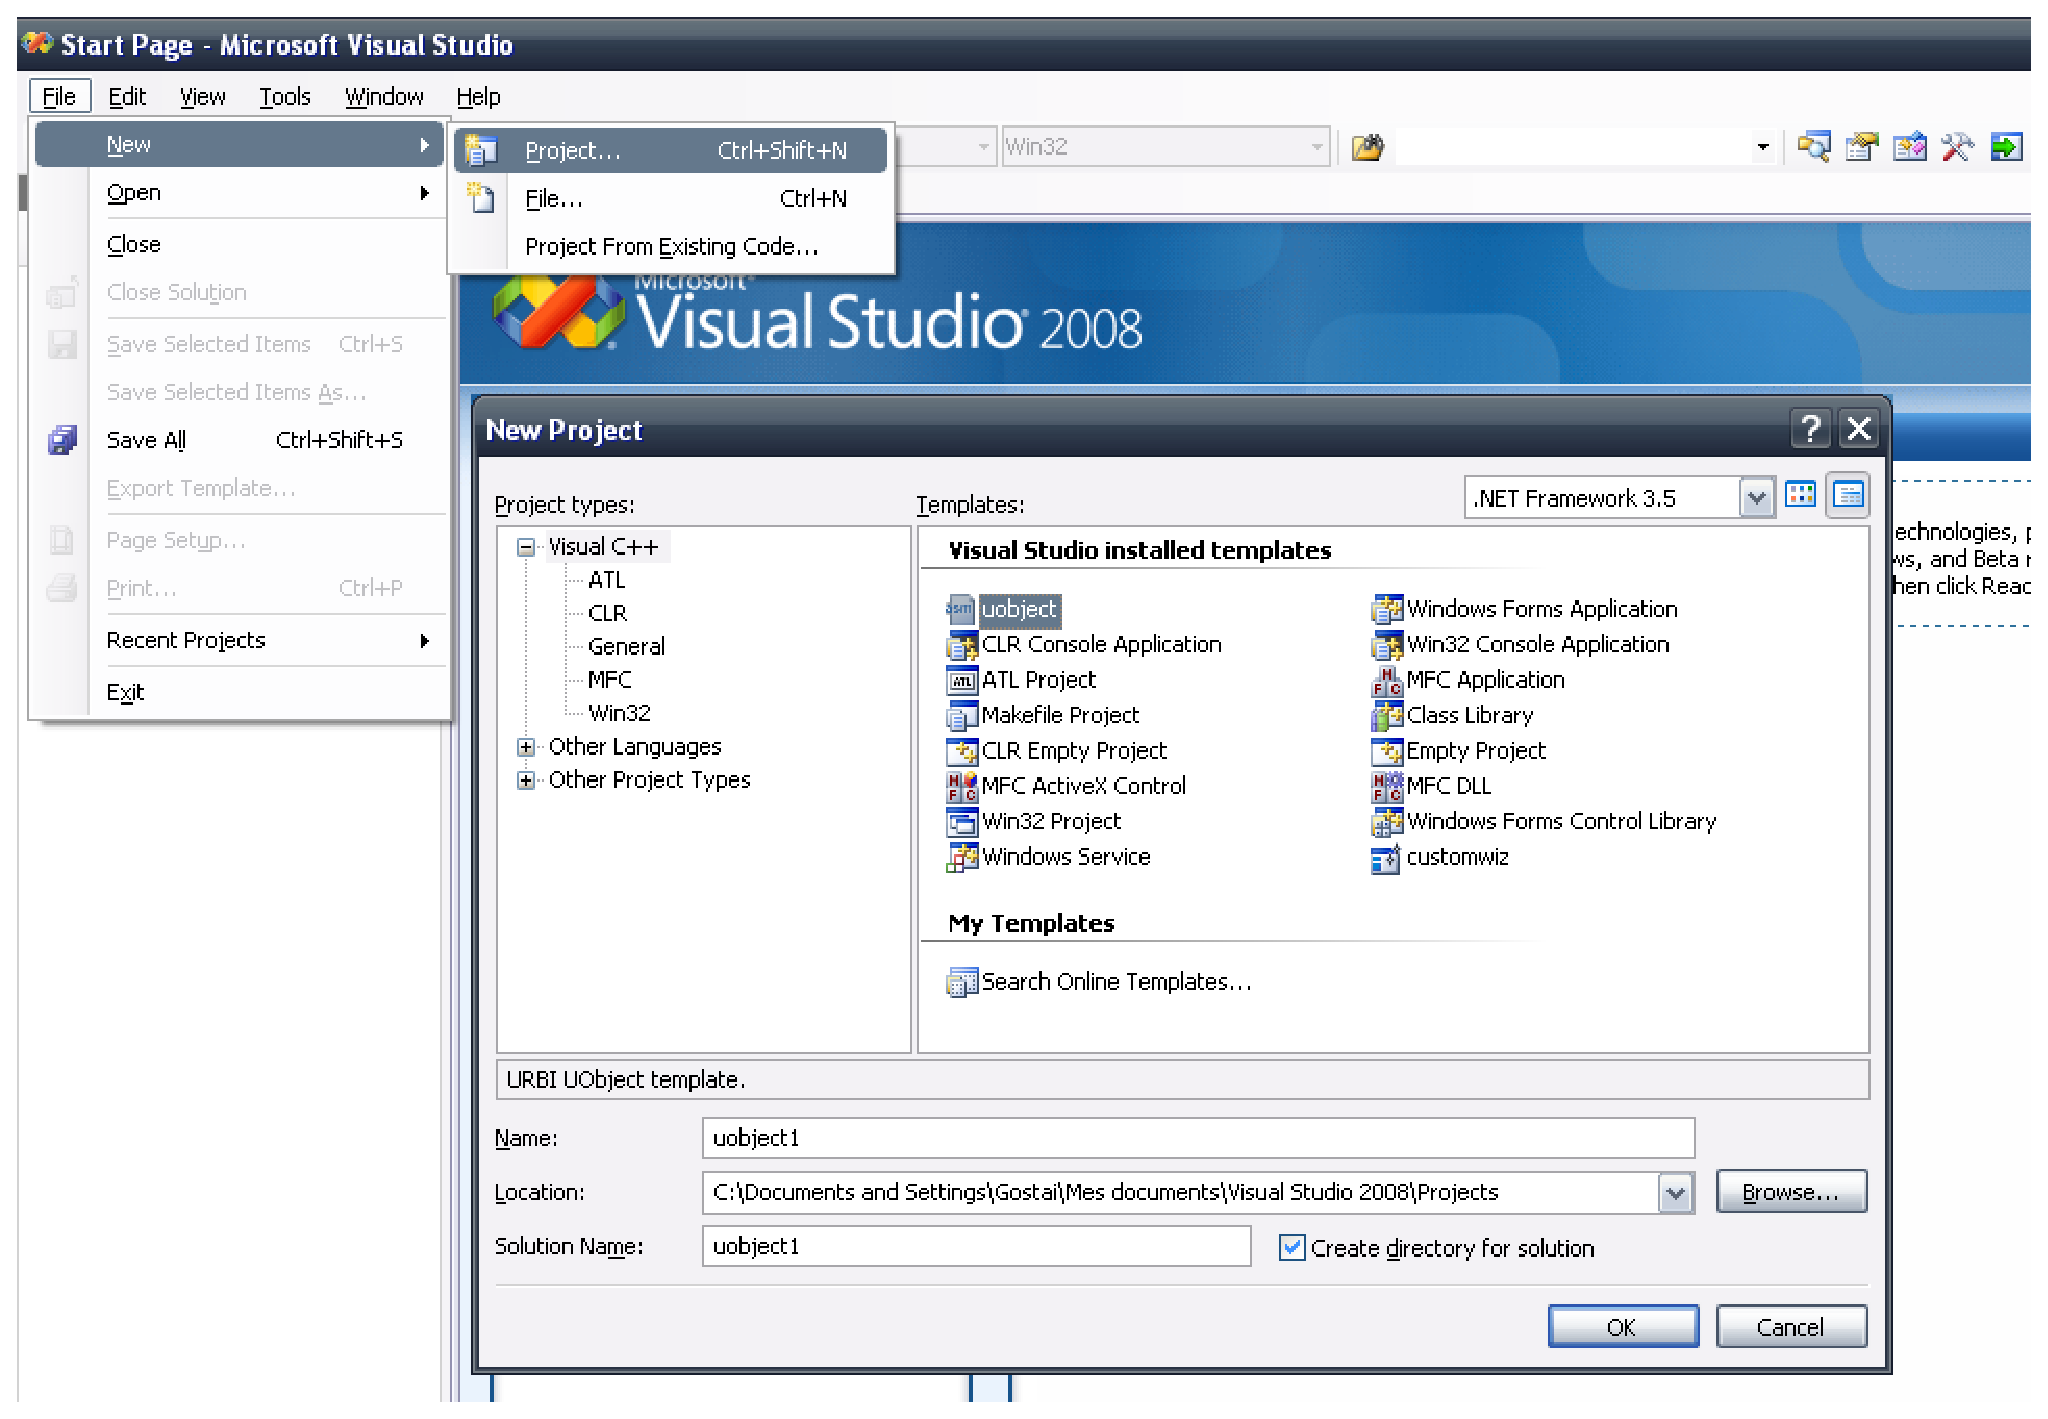
\includegraphics[width=0.6\linewidth]{img/visual-wizard-1}
\end{center}

Then, compile your UObject.

\begin{center}
  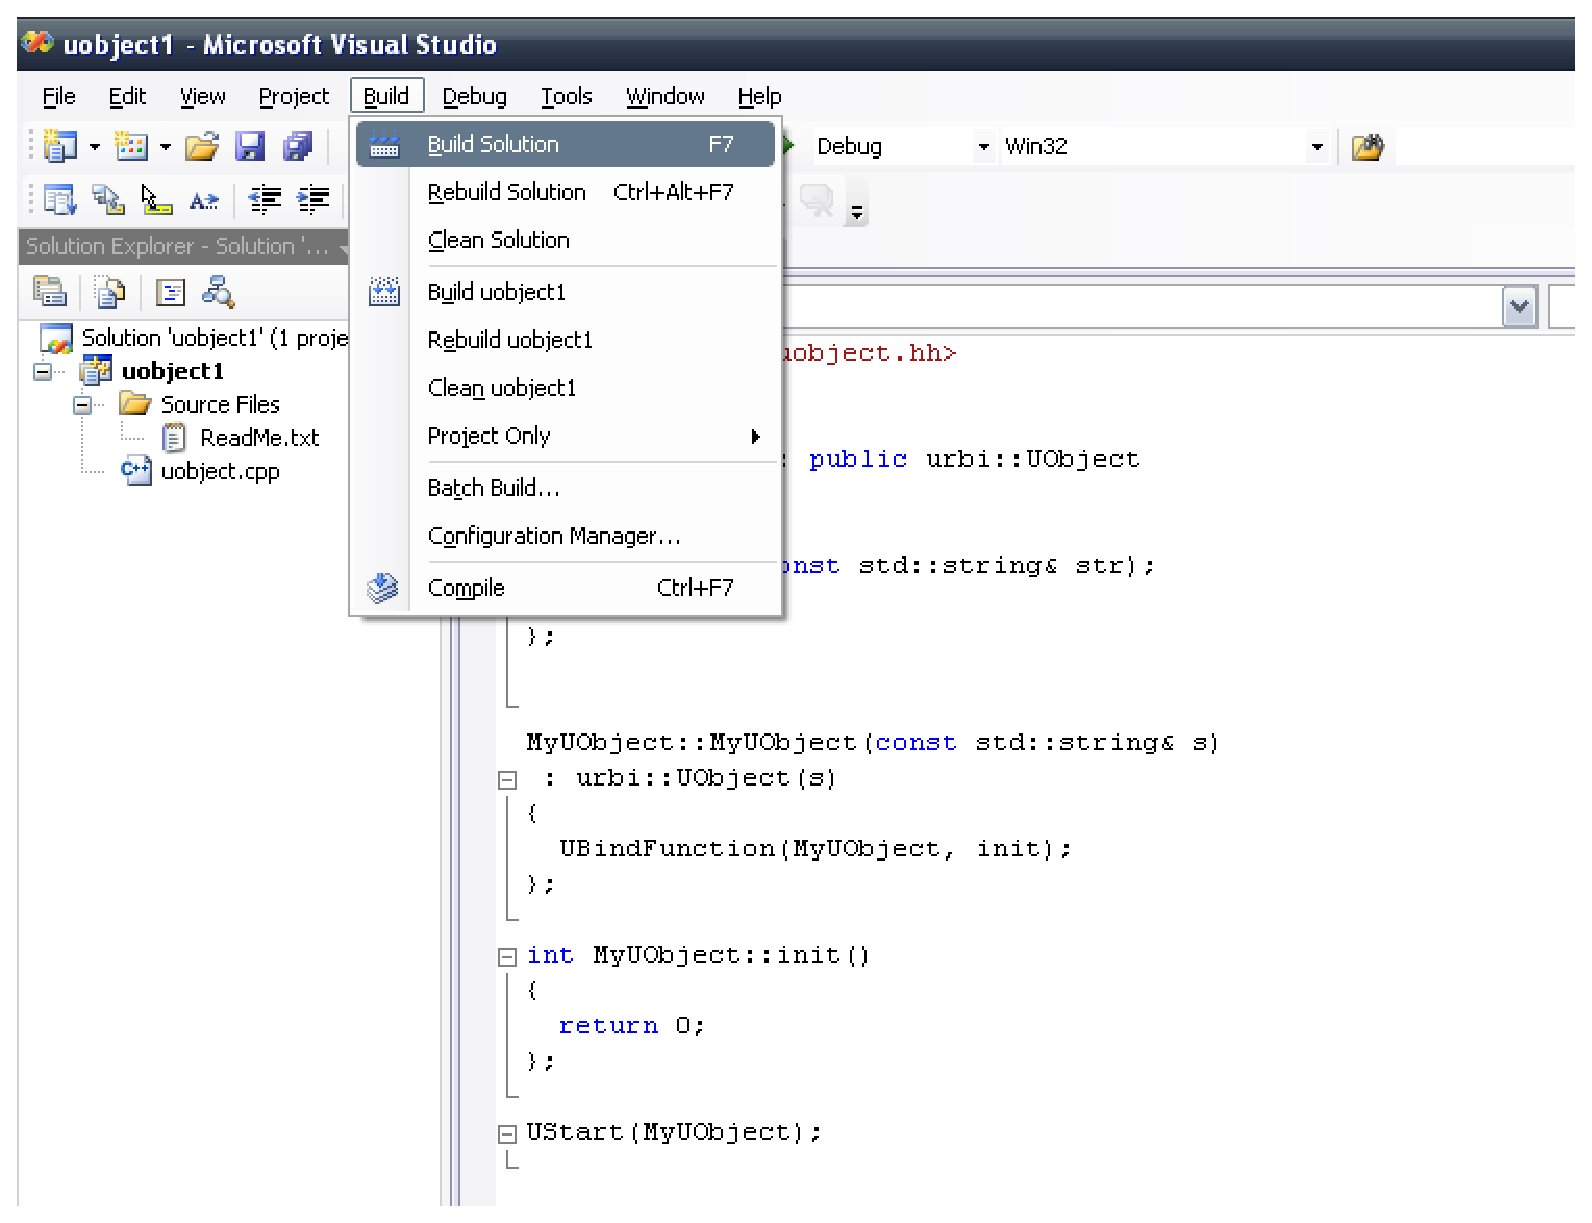
\includegraphics[width=0.6\linewidth]{img/visual-wizard-2}
\end{center}

And run it.

\begin{center}
  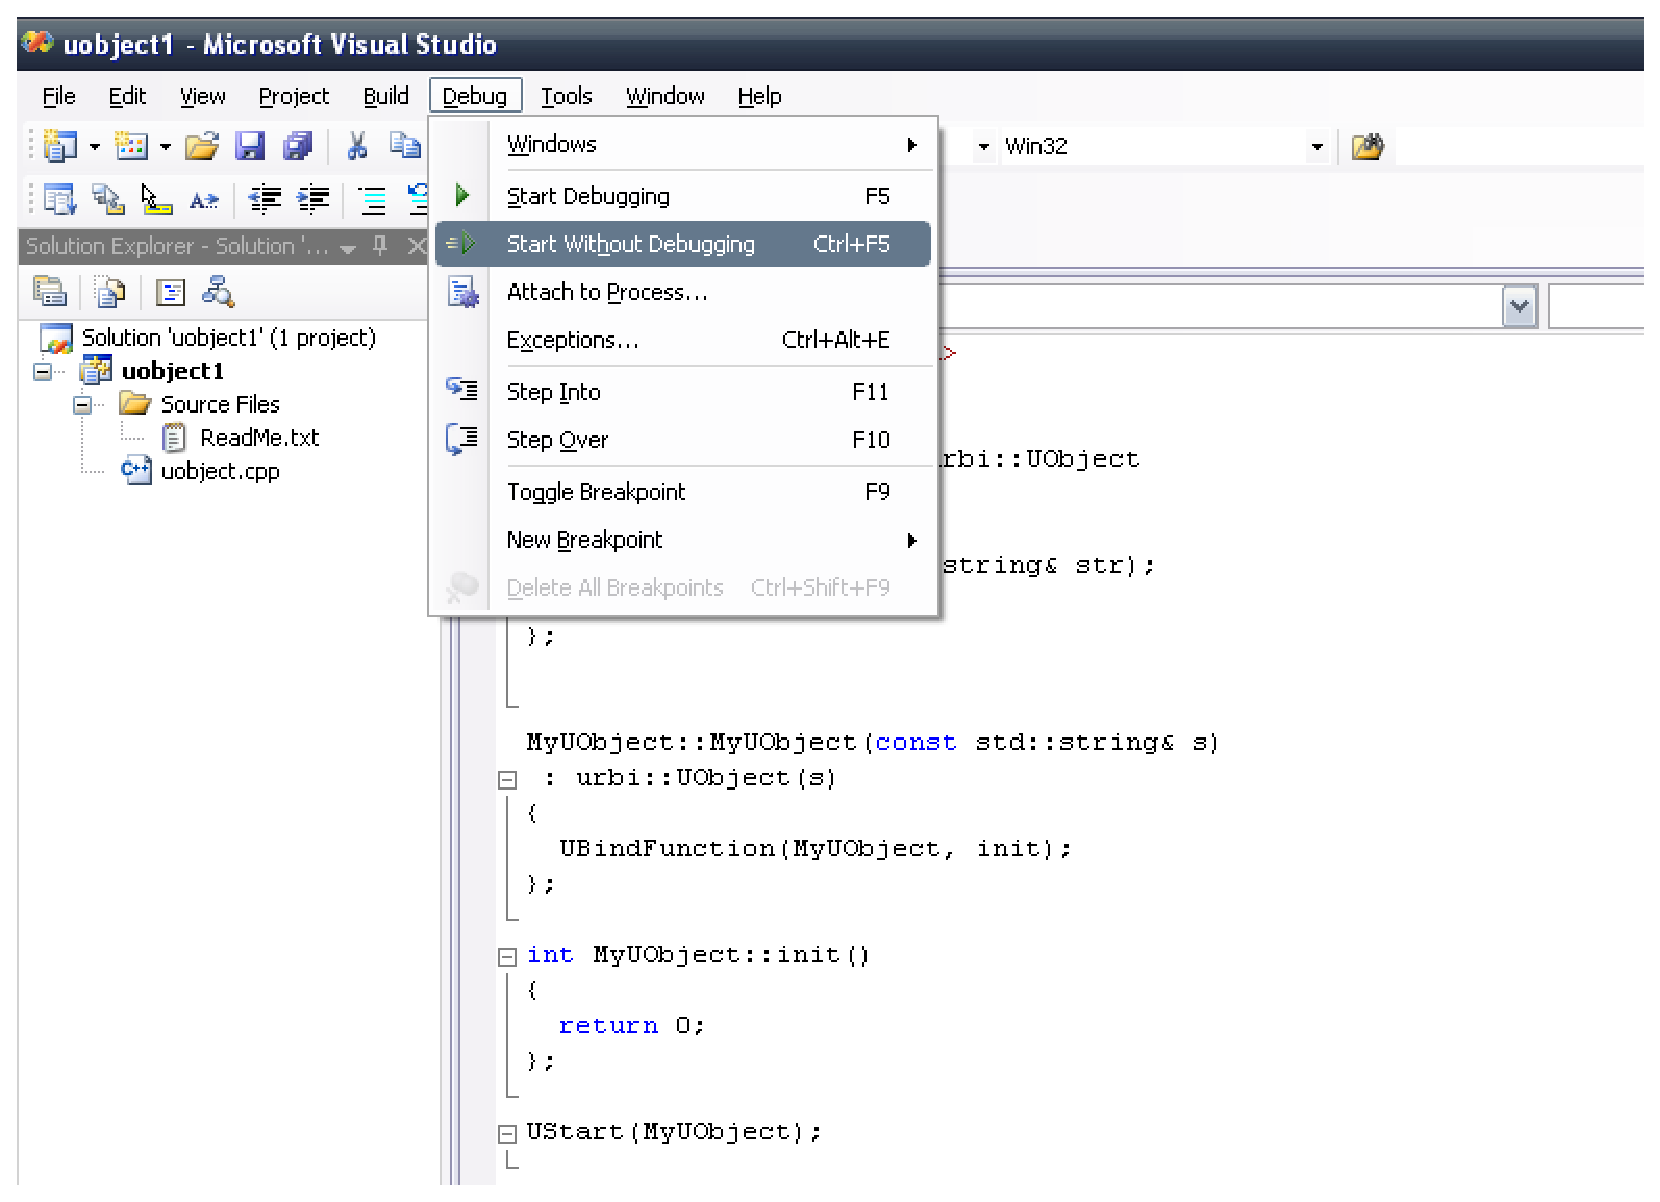
\includegraphics[width=0.6\linewidth]{img/visual-wizard-3}
\end{center}


\section{Creating a class, binding variables and functions}
\label{sec:uob:api:bind}

Let's illustrate those concepts by defining a simple object:
\lstinline{adder}. This object has one variable \lstinline{v}, and a
method \lstinline{add} that returns the sum of this variable and its
argument.

\begin{itemize}
\item First the required include:

\begin{cxx}
#include <urbi/uobject.hh>
\end{cxx}

\item Then we declare our \lstinline{adder} class:
\begin{cxx}
class adder : public urbi::UObject // Must inherit from UObject.
{
  public:
   // The class must have a single constructor taking a string.
   adder (const std::string&);

   // Our variable.
   urbi::UVar v;

   // Our method.
   double add (double);
};
\end{cxx}
\item The implementation of the constructor and our \lstinline{add}
  method:
\begin{cxx}
// the constructor defines what is available from Urbi
adder::adder (const std::string& s)
  : UObject (s) // required
{
  // Bind the variable.
  UBindVar (adder, v);

  // Bind the function.
  UBindFunction (adder, add);
}

double
adder::add (double rhs)
{
  return v + rhs;
}
\end{cxx}
\item And register this class:
\begin{cxx}
// Register the class to the Urbi kernel.
UStart (adder);
\end{cxx}
\end{itemize}

To summarize:

\begin{itemize}
\item Declare your object class as inheriting from
  \lstinline{urbi::UObject}.
\item Declare a single constructor taking a string, and pass this
  string to the constructor of \lstinline{urbi::UObject}.
\item Declare the variables you want to share with \urbi with the type
  \lstinline{urbi::UVar}.
\item In the constructor, use the macros
  \lstinline|UBindVar(\var{class-name}, \var{variable-name})|
  for each \UVar you want as an instance variable, and
  \lstinline|UBindFunction(\var{class-name}, \var{function-name})| for
  each function you want to bind.
\item Call the macro \lstinline{UStart} for each object.
\end{itemize}

\section{Creating new instances}

When you start an \urbi server, an object of each class registered
with \lstinline{UStart} is created with the same name as the
class. New instances can be created from \urbi using the
\lstinline|new| method. For each instance created in \urbi, a
corresponding instance of the \Cxx object is created. You can get the
arguments passed to the constructor by defining and binding a method
named \lstinline|init| with the appropriate number of arguments.

\section{Binding functions}

\subsection{Simple binding}

You can register any member function of your \UObject using the macro

% Fix line wrap.
\lstinline|UBindFunction(\var{class-name}, \var{function-name})|.

Once done, the function can be called from \us.

The following types for arguments and return value are supported:

\begin{itemize}
\item Basic integer and floating types (int, double, float...).
\item \lstinline{const std::string&} or \lstinline{const char*}.
\item \lstinline{urbi::UValue} or any of its subtypes (\UBinary, \UList...).
\item \lstinline{std::list} or \lstinline{std::vector} of the above types.
\end{itemize}

\subsection{Multiple bindings}

If you have multiple functions to bind, you can use the
\lstinline|UBindFunctions| macro to bind multiple functions at once:

\lstinline|UBindFunctions(\var{class-name}, \var{function1}, \var{function2}...)|.

\subsection{Asynchronous binding}
Functions bound using \lstinline{UBindFunction} are called synchronously, and
thus block everything until they return.

If you wish to bind a function that requires a non-negligible amount of time
to execute, you can have it execute in a separate thread by calling

% Separate line since lstinline does not word-wrap and this one is quite long.
\lstinline|UBindThreadedFunction(\var{class-name}, \var{function-name}, \var{lockMode})|.

The function code will be executed in a separate thread without breaking the
\us execution semantics.

The \lstinline{lockMode} argument can be used to prevent parallel execution
of multiple bound functions if your code is not thread-safe. It can be any of
\lstinline{LOCK_NONE}, \lstinline{LOCK_FUNCTION}, \lstinline{LOCK_INSTANCE},
\lstinline{LOCK_CLASS} or \lstinline{LOCK_MODULE}.
When set to \lstinline{LOCK_NONE}, no locking is performed. Otherwise, it
limits parallel executions to:

\begin{itemize}
\item One instance of the bound function for \lstinline{LOCK_FUNCTION}.
\item One bound function for each object instance for
\lstinline{LOCK_INSTANCE}.
\item One bound function for the class for \lstinline{LOCK_CLASS}.
\item One bound function for the whole module (shared object) for
\lstinline{LOCK_MODULE}.
\end{itemize}

There is however a restriction: you cannot mix multiple locking modes: for
instance a function bound with \lstinline{LOCK_FUNCTION} mode will not prevent
another function bound with \lstinline{LOCK_INSTANCE} from executing in
parallel.

You can perform your own locking using semaphores if your code needs a more
complex locking model.

You can limit the maximum number of threads that can run in parallel by using
the \lstinline{setThreadLimit} function.

\section{Notification of a variable change or access}
\label{sec:uobject:uvar-notify}
You can register a function that will be called each time a variable
is modified or accessed (for embedded components only) by calling
\lstinline{UNotifyChange} and \lstinline{UNotifyAccess}, passing
either an \UVar or a variable name as first argument, and a member
function of your \UObject as second argument. This function can take
zero or one argument of any type. If the argument is of type \lstinline{UVar&},
the value will be a reference  to the \UVar being accessed or modified.
If it is of any other type, the system will try to convert the current value
of the \UVar to this type and pass this value to the function.
The \lstinline{notifyChange} callback function
is called after the variable value is changed, whereas the
\lstinline{notifyAccess} callback is called before the variable is
accessed, giving you the possibility to update its value.

Notify functions can be unregistered by calling the
\lstinline|unnotify| function of the \UVar class.

\section{Data-flow based programming: exchanging UVars}

The \lstinline{UNotifyChange} and \lstinline{UNotifyAccess} features
can be used to link multiple UObjects together, and perform data-flow
based programming: the \lstinline{UNotifyChange} can be called to
monitor UVars from other UObjects.  Those UVars can be transmitted
through bound function calls.

One possible pattern is to have each data-processing UObject take its
input from monitored UVars, given in its constructor, and output the
result of its processing in other UVars. Consider the following
example of an object-tracker:

\begin{cxx}
class ObjectTracker: public urbi::UObject
{
  ObjectTracker(const std::string& n)
    : urbi::UObject(n)
  {
    // Bind our constructor.
    UBindFunction(ObjectTracker, init);
  }
  // Take our data source in our constructor.
  void init(UVar& image)
  {
    UNotifyChange(image, &ObjectTracker::onImage);
    // Bind our output variable.
    UBindVar(ObjectTracker, val);
  }
  void onImage(UVar& src)
  {
    UBinary b = src;
    // Processing here.
    val = processing_result;
  }
  UVar val;
};
UStart(ObjectTracker);
\end{cxx}

The following \us code would be used to initialize an ObjectTracker given a
camera:

\begin{urbiunchecked}
var tracker = ObjectTracker.new(camera.getSlot("val"));
\end{urbiunchecked}

An other component could then take the tracker output as its input.

Using this model, chains of processing elements can be created. Each time the
UObject at the start of the chain updates, all the notifyChange will be called
synchronously in cascade to update the state of the intermediate components.

\section{Timers}
\label{sec:uob:timers}

The API provides two methods to have a function called periodically:
\begin{cxxapi}
\item[void urbi::UObject::USetUpdate(ufloat period)]
  Set up a timer that calls the virtual method
  \lstinline{UObject::update()} with the specified period (in
  milliseconds).  Disable updates if \var{period} is -1.

\item[urbi::TimerHandle urbi::UObject::USetTimer<T>(ufloat period, void (T::*fun)())]
  Invoke an UObject member function \var{fun} every \var{period}
  milliseconds.  \var{fun} is a regular member-function pointer, for
  instance \lstinline|MyUObject::my_function|.
  The function returns a \lstinline|TimerHandle| that can be passed to the
  \lstinline|UObject::removeTimer(h)| function to disable the timer.
\end{cxxapi}

\section{The special case of sensor/effector variables}

In \urbi, a variable can have a different meaning depending on whether
you are reading or writing it: you can use the same variable to
represent the target value of an effector and the current value
measured by an associated sensor. This special mode is activated by
the \UObject defining the variable by calling
\lstinline{UOwned} after calling \lstinline{UBindVar}. This call has
the following effects:
\begin{itemize}
\item When \urbi code or code in other modules read the variable, they
  read the current value.
\item When \urbi code or code in other modules write the variable,
  they set the target value.
\item When the module that called \lstinline|UOwned| reads the
  variable, it reads the target value. When it writes the variable, it
  writes the current value.
\end{itemize}

\section{Using \urbi variables}

You can read or write any \urbi variable by creating an
\UVar passing the variable name to the constructor. Change
the value by writing any compatible type to the \UVar, and
access the value by casting the \UVar to any compatible
type.

Some care must be taken in remote mode: changes on the
variable coming from \urbi code or an other module can take time to propagate
to the \UVar. By default, all changes to the value will be sent to the remote
\UObject. To have more control on the bandwidth used, you can
disable the automatic update by calling \lstinline|unnotify()|. Then you can get
the value on demand by calling \lstinline|UVar::syncValue()|.

You can read and write all the \urbi properties of an \UVar by
reading and writing the appropriate \lstinline{UProp} object in the
\UVar.

\section{Emitting events}

The \UEvent class can be used to create and emit \us events. Instances are
created and initialized exactly as \UVar: either by using the
\lstinline{UBindEvent} macro, or by calling one of its constructors or the
\lstinline{init} function.

Once initialized, the \lstinline{emit} function will trigger the emission of
the associated \us event. It can be called with any number of arguments, of
any compatible type.

\section{UObject and Threads}

The \UObject API is thread-safe in both plugin and remote mode: All API calls
including operations on \UVar can be performed from any thread.

\section{Using binary types}

\urbi can store binary objects of any type in a generic container, and
provides specific structures for sound and images. The generic
containers is called \UBinary and is defined in the
\file{urbi/ubinary.hh} header. It contains an enum field type
giving the type of the binary (\lstinline{UNKNOWN}, \lstinline{SOUND}
or \lstinline{IMAGE}), and an union of a \USound and
\UImage struct containing a pointer to the data, the size
of the data and type-specific meta-information.

\subsection{UVar conversion and memory management}
The \UBinary manages its memory: when destroyed (or going out-of-scope), it
frees all its allocated data. The \USound and \UImage do not.

Reading an \UBinary from a \UVar, and writing a
\UBinary, \USound or \UImage to an \UVar performs a deep-copy of the
data (by default, see below).

Reading a \USound or \UImage from an \UVar performs a shallow copy. Modifying
the data is not allowed in that case.

\subsection{0-copy mode}
In plugin mode, you can setup any \UVar in 0-copy mode by calling
\lstinline{setBypass(true)}. In this mode, binary data written to the \UVar
is not copied, but a reference is kept.
As a consequence, the data is only available from within registered
notifyChange callbacks. Those callbacks can use \lstinline|UVar::val()| or
cast the \UVar to a \UBinary\& to retrieve the reference.
Attempts to read the \UVar from outside notifyChange will result in
\lstinline{nil} being returned.

\section{Using hubs to group objects}

Sometimes, you need to perform actions for a group of
\lstinline{UObjects}, for instance devices that need to be updated
together. The API provides the \UObjectHub class for this
purpose. To create a hub, simply declare a subclass of
\UObjectHub, and register it by calling once the macro
\lstinline|UStartHub (\var{class-name})|. A single instance of this class
will then be created upon server start-up. \UObject
instances can then register to this hub by calling
\lstinline|URegister (\var{hub-class-name})|. Timers can be attached to
\UObjectHub the same way as to \UObject (see
\autoref{sec:uob:timers}). The kernel will call the \lstinline{update()}
method of all \UObject before calling the
\lstinline{update()} method of the hub. A hub instance can be
retrieved by calling \lstinline{getUObjectHub (string classname)}. The
hub also holds the list of registered UObject in its members
attribute.

\section{Sending \us code}

If you need to send \us code to the server, the \lstinline{URBI()}
macro is available, as well as the \lstinline{send()} function. You
can either pass it a string, or directly \urbi code inside a double
pair of parentheses:

\begin{urbiunchecked}
send ("myTag:1+1;");

URBI (( at (myEvent?(var x)) { myTag:echo x; }; ));
\end{urbiunchecked}

You can also use the \lstinline{call} method to make an urbiscript function
call:

\begin{urbiunchecked}
// C++ equivalent of urbiscript 'System.someFunc(12, "foo");'
call("System", "someFunc", 12, "foo");
\end{urbiunchecked}

\section{Using RTP transport in remote mode}
\label{sec:uob:api:rtp}

By default, \urbi uses TCP connections for all communications between the
engine and remote UObjects. \urbi also supports the UDP-based \dfn{RTP}
protocol for more efficient transmission of updated variable values. RTP
will provide a lower latency at the cost of possible packet loss, especially
in bad wireless network conditions.

\subsection{Enabling RTP}

To enable RTP connections, both the engine and the remote-mode urbi-launch
containing your remote \UObject must load the RTP \UObject. This can be
achieved by passing \lstinline|urbi/rtp| as an extra argument to both
urbi-launch command lines (one for the engine, the other for your remote
\UObject).

Once done, all binary data transfer (like sound and image) in both
directions will by default use a RTP connection.

\subsection{Per-UVar control of RTP mode}

You can control whether a specific \UVar uses RTP mode by calling its
\lstinline|useRTP(bool)| function. Each binary-type \UVar will have its own
RTP connection, and all non-binary \UVar will share one.

%%% Local Variables:
%%% mode: latex
%%% TeX-master: "../urbi-sdk"
%%% ispell-dictionary: "american"
%%% ispell-personal-dictionary: "../urbi.dict"
%%% fill-column: 76
%%% End:

%% Copyright (C) 2009-2010, Gostai S.A.S.
%%
%% This software is provided "as is" without warranty of any kind,
%% either expressed or implied, including but not limited to the
%% implied warranties of fitness for a particular purpose.
%%
%% See the LICENSE file for more information.

\chapter{Use Cases}
\label{sec:uob:uses}
\section{Writing a Servomotor Device}

Let's write a \lstinline{UObject} for a servomotor device whose
underlying API is:

\begin{cxxapi}
\item[bool initialize (int id)]
  Initialize the servomotor with given ID.
\item[double getPosition (int id)]
  Read servomotor of given id position.
\item[void setPosition (int id, double pos)]
  Send a command to servomotor.
\item[void setPID (int id, int p, int i, int d)]
  Set P, I, and D arguments.
\end{cxxapi}

First our header. Our servo device provides an attribute named
\lstinline{val}, the standard \urbi name, and two ways to set PID
gain: a method, and three variables.

\begin{cxx}
class servo : public urbi::UObject // must inherit UObject
{
public:
  // the class must have a single constructor taking a string
  servo(const std::string&);

  // Urbi  constructor
  void init(int id);

  // main attribute
  urbi::UVar val;

  // position variables:
  //  P gain
  urbi::UVar P;
  //  I gain
  urbi::UVar I;
  //  D gain
  urbi::UVar D;

  // callback for val change
  void valueChanged(UVar& v);
  //callback for val access
  void valueAccessed(UVar& v);
  // callback for PID change
  void pidChanged(UVar& v);

  // method to change all values
  void setPID(int p, int i, int d);

  // motor ID
  int id_;
};
\end{cxx}

The constructor only registers init, so that our default instance
\lstinline{servo} does nothing, and can only be used to create new
instances.

\begin{cxx}
servo::servo (const std::string& s)
  : urbi::UObject (s)
{
   // register init
   UBindFunction (servo, init);
}
\end{cxx}

The \lstinline{init} function, called in a new instance each time a
new \urbi instance is created, registers the four variables
(\lstinline{val}, \lstinline{P}, \lstinline{I} and \lstinline{D}), and
sets up callback functions.

\begin{cxx}
// Urbi constructor.
void
servo::init (int id)
{
  id_ = id;

  if (!initialize (id))
    return 1;

  UBindVar (servo, val);

  // val is both a sensor and an actuator.
  Uowned (val);

  // Set blend mode to mix.
  val.blend = urbi::UMIX;

  // Register variables.
  UBindVar (servo, P);
  UBindVar (servo, I);
  UBindVar (servo, D);

  // Register functions.
  UBindFunction (servo, setPID);

  // Register callbacks on functions.
  UNotifyChange (val, &servo::valueChanged);
  UNotifyAccess (val, &servo::valueAccessed);
  UNotifyChange (P, &servo::pidChanged);
  UNotifyChange (I, &servo::pidChanged);
  UNotifyChange (D, &servo::pidChanged);
}
\end{cxx}

Then we define our callback methods. \lstinline{servo::valueChanged}
will be called each time the \lstinline{val} variable is modified,
just after the value is changed: we use this method to send our servo
commands. \lstinline{servo::valueAccessed} is called just before the
value is going to be read. In this function we request the current
value from the servo, and set \lstinline{val} accordingly.

\begin{cxx}
// Called each time val is written to.
void
servo::valueChanged (urbi::UVar& v)
{
  // v is a reference to our class member val: you can use both
  // indifferently.
  setPosition (id, (double)val);
}

// Called each time val is read.
void
servo::valueAccessed (urbi::UVar& v)
{
  // v is a reference to val.
  val = getPosition (id);
}
\end{cxx}

\lstinline{servo::pidChanged} is called each time one of the PID
variables is written to. The function \lstinline{servo::setPID} can be
called directly from \urbi.

\begin{cxx}
void
servo::pidChanged (urbi::UVar& v)
{
  setPID(id, (int)P, (int)I, (int)D);
}

void
servo::setPID (int p, int i, int d)
{
  setPID (id, p, i, d);
  P = p;
  I = i;
  D = d;
}

// Register servo class to the Urbi kernel.
UStart (servo);
\end{cxx}

That's it, compile this module, and you can use it within \us:

\begin{urbiunchecked}
// Create a new instance.  Calls init (1).
headPan = new servo (1);

// Calls setPID ().
headPan.setPID (8,2,1);

// Calls valueChanged ().
headPan.val = 13;

// Calls valueAccessed ().
headPan.val * 12;

// Periodically calls valueChanged ().
headPan.val = 0 sin:1s ampli:20,

// Periodically calls valueAccessed ().
at (headPan.val < 0)
  echo ("left");
\end{urbiunchecked}

The sample code above has one problem: \lstinline{valueAccessed} and
\lstinline{valueChanged} are called each time the value is read or
written from \urbi, which can happen quite often. This is a problem if
sending the actual command (\lstinline{setPosition} in our example)
takes time to execute. There are two solutions to this issue.

\subsection{Caching}

One solution is to remember the last time the value was read/written,
and not apply the new command before a fixed time. Note that the
kernel is doing this automatically for \lstinline{UOwned}'d variables
that are in a blend mode different than \lstinline{normal}. So the
easiest solution to the above problem is likely to set the variable to
the \lstinline{mix} blending mode. The unavoidable drawback is that
commands are not applied immediately, but only after a small delay.

\subsection{Using Timers}

Instead of updating/fetching the value on demand, you can chose to do
it periodically based on a timer. A small difference between the two
API methods comes in handy for this case: the \lstinline{update()}
virtual method called periodically after being set up by
\lstinline{USetUpdate(interval)} is called just after one pass of
\urbi code execution, whereas the timers set up by
\lstinline{USetTimer} are called just before one pass of \urbi code
execution. So the ideal solution is to read your sensors in the second
callback, and write to your actuators in the first. Our previous
example (omitting PID handling for clarity) can be rewritten. The
header becomes:

\begin{cxx}
// Inherit from UObject.
class servo : public urbi::UObject
{
public:
  // The class must have a single constructor taking a string.
  servo (const std::string&)

  // Urbi constructor.
  void init (int id);

  // Called periodically.
  virtual int update ();
  // Called periodically.
  void getVal ();

  // Our position variable.
  urbi::UVar val;

  // Motor ID.
  int id_;
};
\end{cxx}

Constructor is unchanged, \lstinline{init} becomes:

\begin{cxx}
// Urbi constructor.
void
servo::init (int id)
{
  id_ = id;

  if (!initialize (id))
    return 0;

  UBindVar (servo,val);
  // Val is both a sensor and an actuator.
  UOwned(val);

  // Will call update () periodically.
  USetUpdate(1);
  // Idem for getVal ().
  USetTimer (1, &servo::getVal);
}
\end{cxx}

\lstinline{valueChanged} becomes \lstinline{update} and
\lstinline{valueAccessed} becomes \lstinline{getVal}. Instead of being
called on demand, they are now called periodically. The period of the
call cannot be lower than the value returned by
\lstinline{Object.getPeriod;}
so you can set it to 0 to mean ``as fast as is useful''.

\section{Using Hubs to Group Objects}

Now, suppose that, for our previous example, we can speed things up by
sending all the servomotor commands at the same time, using the
following method that takes two arrays of ids and positions.

\begin{cxx}
void setPositions(int count, int* ids, double* positions);
\end{cxx}

A hub is the perfect way to handle this task. The UObject header stays
the same. We add a hub declaration:

\begin{cxx}
class servohub : public urbi::UObjectHub
{
public:
  // The class must have a single constructor taking a string.
  servohub (const std::string&);

  // Called periodically.
  virtual int update ();

  // Called by servo.
  void addValue (int id, double val);

  int* ids;
  double* vals;
  int size;
  int count;
};
\end{cxx}

\lstinline{servo::update} becomes a call to the \lstinline{addValue}
method of the hub:

\begin{cxx}
int
servo::update()
{
  ((servohub*)getUObjectHub ("servohub"))->addValue (id, (double)val);
};
\end{cxx}

The following line can be added to the servo \lstinline{init} method,
although it has no use in our specific example:

\begin{cxx}
URegister(servohub);
\end{cxx}

Finally, the implementation of our hub methods is:

\begin{cxx}
servohub::servohub (const std::string& s)
  : UObjectHub (s)
  , ids   (0)
  , vals  (0)
  , size  (0)
  , count (0)
{
  // setup our timer
  USetUpdate (1);
}

int
servohub::update ()
{
  // Called periodically.
  setPositions (count, ids, vals);

  // Reset position counter.
  count = 0;

  return 0;
}

void
servohub::addValue (int id, double val)
{
  if (count + 1 < size)
  {
    // Allocate more memory.
    ids = (int*) realloc (ids, (count + 1) * sizeof (int));
    vals = (double*) realloc (vals, (count + 1) * sizeof (double));
    size = count + 1;
  }
  ids[count] = id;
  vals[count++] = val;
}

UStartHub (servohub);
\end{cxx}

Periodically, the \lstinline{update} method is called on each servo
instance, which adds commands to the hub arrays, then the
\lstinline{update} method of the hub is called, actually sending the
command and resetting the array.

\subsection{Alternate Implementation}

Alternatively, to demonstrate the use of the members hub variable, we
can entirely remove the \lstinline{update} method in the servo class
(and the \lstinline{USetUpdate()} call in \lstinline{init}), and
rewrite the hub \lstinline{update} method the following way:

\begin{cxx}
int servohub::update()
{
  //called periodically
  for (UObjectList::iterator i = members.begin ();
       i != members.end ();
       ++i)
    addValue (((servo*)*i)->id, (double)((servo*)*i)->val);
  setPositions(count, ids, vals);
  // reset position counter
  count = 0;

  return 0;
}
\end{cxx}

\section{Writing a Camera Device}

A camera device is an UObject whose \lstinline{val} field is a binary
object. The \urbi kernel itself doesn't make any difference between
all the possible binary formats and data type, but the API provides
image-specific structures for convenience. You must be careful about
memory management. The \lstinline{UBinary} structure handles its own
memory: copies are deep, and the destructor frees the associated
buffer. The \lstinline{UImage} and \lstinline{USound} structures do
not.

Let's suppose we have an underlying camera API with the following functions:
\begin{cxxapi}
\item[bool initialize (int id)]\\
  Initialize the camera with given ID.
\item[int getWidth (int id)]\\
  Return image width.
\item[int getHeight (int id)]\\
  Return image height.
\item[char* getImage (int id)]\\
  Get image buffer of format RGB24.  The buffer returned is always the
  same and doesn't have to be freed.
\end{cxxapi}

Our device code can be written as follows:
\begin{cxx}
// Inherit from UObject.
class Camera : public urbi::UObject
{
public:
  // The class must have a single constructor taking a string.
  Camera(const std::string&);

  // Urbi constructor. Throw in case of error.
  void init (int id);

  // Our image variable and dimensions.
  urbi::UVar val;
  urbi::UVar width;
  urbi::UVar height;

  // Called on access.
  void getVal (UVar&);

  // Called periodically.
  virtual int update ();

  // Frame counter for caching.
  int frame;
  // Frame number of last access.
  int accessFrame;
  // Camera id.
  int id_;
  // Storage for last captured image.
  UBinary bin;
};
\end{cxx}

The constructor only registers \lstinline{init}:

\begin{cxx}
Camera::Camera (const std::string& s)
  : urbi::UObject (s)
  , frame (0)
{
  UBindFunction (Camera, init);
}
\end{cxx}

The \lstinline{init} function binds the variable, a function called on
access, and sets a timer up on update. It also initializes the
\lstinline{UBinary} structure.

\begin{cxx}
void
Camera::init (int id)
{
  //urbi constructor
  id_ = id;
  frame = 0;
  accessFrame = 0;

  if (!initialize (id))
    throw std::runtime_error("Failed to initialize camera");

  UBindVar (Camera, val);
  UBindVar (Camera, width);
  UBindVar (Camera, height);
  width = getWidth (id);
  height = getHeight (id);

  UNotifyAccess (val, &Camera::getVal);

  bin.type = BINARY_IMAGE;
  bin.image.width = width;
  bin.image.height = height;
  bin.image.imageFormat = IMAGE_RGB;
  bin.image.size = width * height * 3;

  // Call update () periodically.
  USetUpdate (1);
}
\end{cxx}

The \lstinline{update} function simply updates the frame counter:

\begin{cxx}
int
Camera::update ()
{
  ++frame;
  return 0;
}
\end{cxx}

The \lstinline{getVal} updates the camera value, only if it hasn't
already been called this frame, which provides a simple caching
mechanism to avoid performing the potentially long operation of
acquiring an image too often.

\begin{cxx}
void
Camera::getVal(urbi::UVar&)
{
  if (frame == accessFrame)
    return;

  bin.image.data = getImage (id);
  // Assign image to bin.
  val = bin;
}

UStart(Camera);
\end{cxx}

The image data is copied inside the kernel when proceeding this way.

Be careful, suppose that we had created the \lstinline{UBinary}
structure inside the \lstinline{getVal} method, our buffer would have
been freed at the end of the function. To avoid this, set it to 0
after assigning the \lstinline{UBinary} to the \lstinline{UVar}.

\subsection{Optimization in Plugin Mode}

In plugin mode, it is possible to access the buffer used by the kernel
by casting the \lstinline{UVar} to a \lstinline{UImage}. You can
modify the content of the kernel buffer but no other argument.

\section{Writing a Speaker or Microphone Device}

Sound handling works similarly to image manipulation, the
\lstinline{USound} structure is provided for this purpose. The
recommended way to implement a microphone is to fill the
\lstinline{UObject} val variable with the sound data corresponding to
one kernel period. If you do so, the \urbi code
\lstinline{loop tag:micro.val,} will produce the expected result.

\section{Writing a Softdevice: Ball Detection}

Algorithms that require intense computation can be written in \Cxx but
still be usable within \urbi: they acquire their data using
\lstinline{UVar} referencing other modules' variables, and output
their results to other \lstinline{UVar}. Let's consider the case of a
ball detector device that takes an image as input, and outputs the
coordinates of a ball if one is found.

The header is defined like:

\begin{cxx}
class BallTracker : public urbi::UObject
{
public:
  BallTracker (const std::string&);
  void init (const std::string& varname);

  // Is the ball visible?
  urbi::UVar visible;

  // Ball coordinates.
  urbi::UVar x;
  urbi::UVar y;
 };
\end{cxx}

The constructor only registers \lstinline{init}:

\begin{cxx}
// The constructor registers init only.
BallTracker::BallTracker (const::string& s)
  : urbi::UObject (s)
{
  UBindFunction (BallTracker, init);
}
\end{cxx}

The \lstinline{init} function binds the variables and a callback on
update of the image variable passed as a argument.

\begin{cxx}
void
BallTracker::init (const std::string& cameraval)
{
  UBindVar (BallTracker, visible);
  UBindVar (BallTracker, x);
  UBindVar (BallTracker, y);
  UNotifyChange (cameraval, &BallTracker::newImage);

  visible = 0;
}
\end{cxx}

The \lstinline{newImage} function runs the detection algorithm on the
image in its argument, and updates the variables.

\begin{cxx}
void
BallTracker::newImage (urbi::UVar& v)
{
  // Cast to UImage.
  urbi::UImage i = v;
  int px,py;
  bool found = detectBall (i.data, i.width, i.height, &px, &py);

  if (found)
  {
    visible = 1;
    x = px / i.width;
    y = py / i.height;
  }
  else
    visible = 0;
}
\end{cxx}

%%% Local Variables:
%%% coding: utf-8
%%% mode: latex
%%% TeX-master: "../urbi-sdk"
%%% ispell-dictionary: "american"
%%% ispell-personal-dictionary: "../urbi.dict"
%%% fill-column: 76
%%% End:


%%% Local Variables:
%%% mode: latex
%%% TeX-master: "../urbi-sdk"
%%% End:

% LocalWords:  UObject API UVar UBinary USound UImage liburbi UValue namespace
% LocalWords:  urbi const UBindVar UBindFunction rhs UStart init UNotifyChange
% LocalWords:  UNotifyAccess notifyChange notifyAccess USetUpdate USetTimer pos
% LocalWords:  UOwned UNotifyOnRequest requestValue UProp enum struct plugin px
% LocalWords:  UObjects UObjectHub UStartHub URegister getUObjectHub classname
% LocalWords:  someevent sometag bool getPosition setPosition setPID PID Uowned
% LocalWords:  valueChanged valueAccessed pidChanged headPan ampli getVal vals
% LocalWords:  setPositions servohub addValue realloc sizeof destructor RGB py
% LocalWords:  getWidth getHeight getImage accessFrame softdevice BallTracker
% LocalWords:  varname cameraval newImage detectBall
